\documentclass{article}
\usepackage{amsmath}
\usepackage{ctex}
\usepackage{graphicx}
\usepackage{circuitikz}

\title{电路第二章作业}
\author{自实陈嘉宇U202414389}
\date{}
\begin{document}
\maketitle
\section*{2-1}电路如图所示,已知$u_s=100V,R_1=2k\Omega,R_2=8k\Omega$.
试求以下三种情况下的电压$u_2$和电流$i_2$,$i_3$:\\
(1)$R_3=8k\Omega$\quad(2)$R_3=\infty$($R_3$开路)
(3)$R_3=0$($R_3$短路).\\
\begin{center}
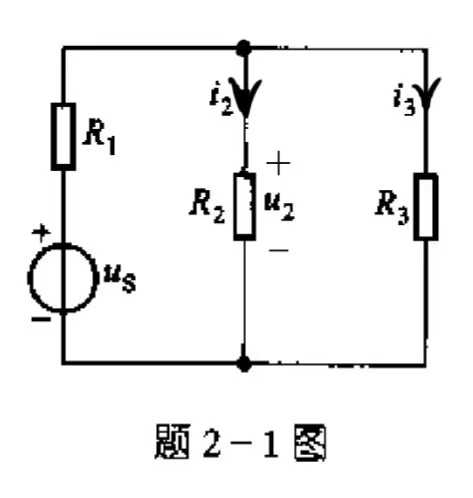
\includegraphics[width=0.4\textwidth,height=0.2\textheight]{2-1.jpg}
\end{center}

\noindent 解:
(1)$R_\text{23}=\frac{R_2R_3}{R_2+R_3}=4k\Omega$,$u_2=u_s\frac{R_\text{23}}{R_1+R_\text{23}}=\frac{200}{3}V$
,$i_2=i_3=\frac{u_2}{R_2}=\frac{1}{12}mA$

(2)$u_2=u_s\frac{R_2}{R_1+R_2}=80V$,$i_2=0.01A$,$i_3=0$

(3)$u_2=0$,$i_2=0$,$i_3=\frac{u_s}{R_1}=0.05A$
\section*{2-2}电路如图所示,其中电阻、电压源和电流源均为已知,且为正值,求:
(1)$u_2$和$i_2$\quad (2)若$R_1$增大,对哪些元件的电压、电流有什么影响?\\
\begin{center}
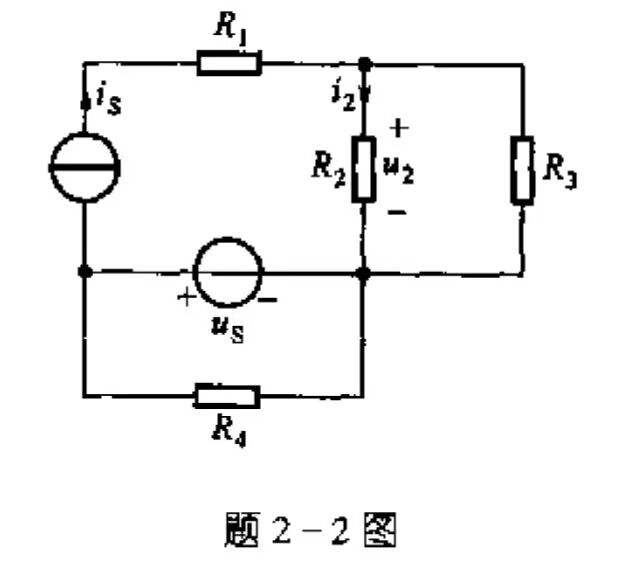
\includegraphics[width=0.4\textwidth,height=0.2\textheight]{2-2.jpg}
\end{center}

\noindent 解:
(1)$u_2=i_s\frac{R_2R_3}{R_2+R_3}$,$i_2=\frac{u_2}{R_2}=i_s\frac{R_3}{R_2+R_3}$

(2)$R_1$增大,$u_1$增大,$i_1$增大,$u_2$减小,$i_2$减小.对电阻$R_4$没有影响.
\section*{2-5}
用$\Delta$-Y等效变换法求图中a,b端的等效电阻:\\
(1)将节点1,2,3之间的3个$9\Omega$电阻用$\Delta$-Y变换成Y型电阻\\
(2)将节点1,3,4与作为内部公共节点的2之间的3个$9\Omega$电阻构成的Y型变换为$\Delta$型\\
\begin{center}
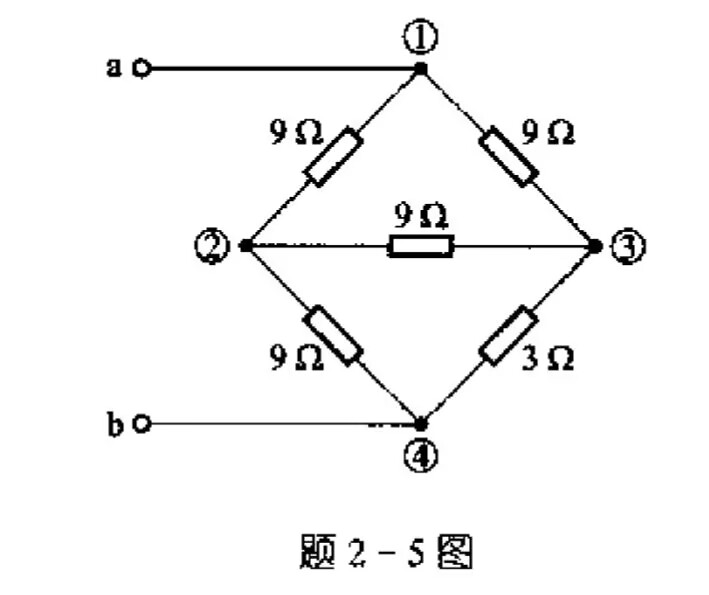
\includegraphics[width=0.4\textwidth,height=0.2\textheight]{2-5.jpg}
\end{center}

\noindent 解:
(1)$R_\text{ab}=(3+\frac{12\times6}{12+6})\Omega=7\Omega$


(2)\(R_\text{ab}=\frac{1}{\frac{1}{27}+\frac{1}{\frac{9\times27}{9+27}+\frac{3\times27}{3+27}}}\Omega=7\Omega\)
\section*{2-7}图(a)所示电路中,
$u_\text{s1}=24V$,$u_\text{s2}=6V$,$R_1=12k\Omega$,$R_2=6k\Omega$,$R_3=2k\Omega$
图(b)为经电源变换后的等效电路。\\
(1)求等效电路的$i_s$和$R$;\\(2)根据等效电路求$R_3$中电流和消耗功率;
\\(3)分别在图(a)(b)中求出$R_1$,$R_2$及$R_3$消耗的功率;
\\(4)试问$u_\text{s1}{s2}$发出的功率是否等于$i_s$发出的功率?$R_1$,$R_2$消耗的功率是否等于$R$消耗的功率?为什么?
\begin{center}
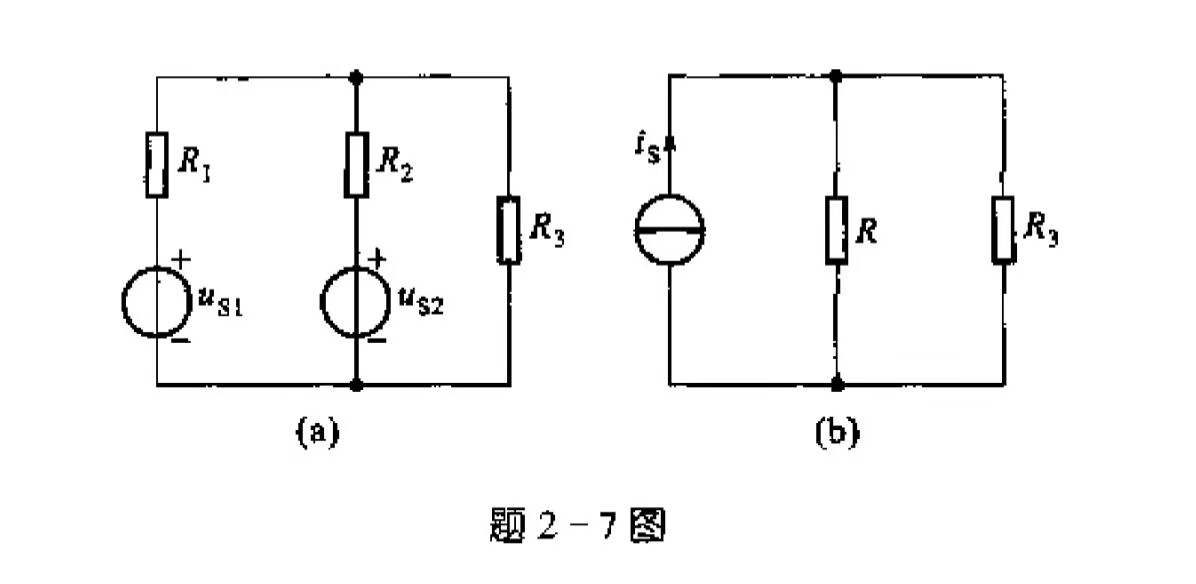
\includegraphics[width=0.7\textwidth,height=0.2\textheight]{2-7.jpg}
\end{center}

\noindent 解:
(1)$i_s=\frac{u_\text{s1}}{R_1}+\frac{u_\text{s=}}{R_2}=3mA$,
$R=R_1//R_2=4k\Omega$

(2)$i_\text{R3}=\frac{R}{R+R_3}=2mA$,$P_\text{R3}=i_\text{R3}^2R_3=8mW$

(3)在图(a)中,$u_\text{R3}=2k\Omega\times2mA=4V$,则
$u_1=u_\text{s1}-u_\text{R3}=20V$,$u_2=u_\text{R2}-u_\text{R3}=2V$
故$P_1=\frac{u_1^2}{R_1}=\frac{1}{30}W$,
$P_2=\frac{u_2^2}{R_2}=\frac{2}{3}mW$,
$P_3=\frac{u_\text{R3}^2}{R_3}=8mW$\\
在图(b)中,等效电源发出功率$12mW$,等效电阻消耗功率$4mW$,由(2)$R_3$消耗功率$8mW$

(4)不相等,等效变换是对外部等效,被变换部分内部不一定等效.
\section*{2-10}
利用电源等效变换求图(a)(b)中电压$u_\text{ab}$
\begin{center}
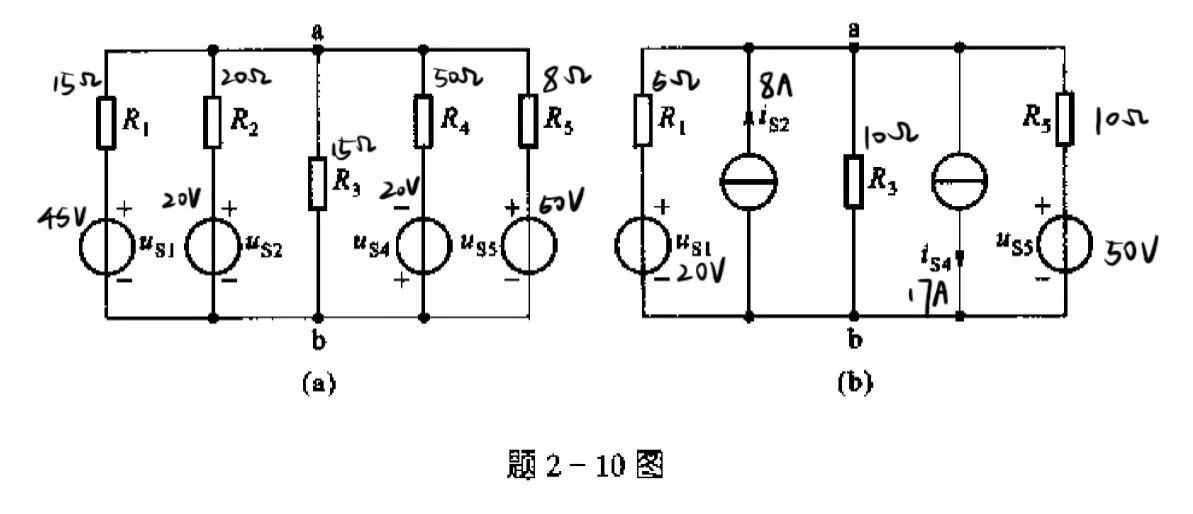
\includegraphics[width=0.7\textwidth,height=0.2\textheight]{2-10.jpg}
\end{center}
To be continued...
\end{document}